\documentclass[11pt,a4paper]{article}\usepackage[]{graphicx}\usepackage[]{color}
% maxwidth is the original width if it is less than linewidth
% otherwise use linewidth (to make sure the graphics do not exceed the margin)
\makeatletter
\def\maxwidth{ %
  \ifdim\Gin@nat@width>\linewidth
    \linewidth
  \else
    \Gin@nat@width
  \fi
}
\makeatother

\definecolor{fgcolor}{rgb}{0.345, 0.345, 0.345}
\makeatletter
\@ifundefined{AddToHook}{}{\AddToHook{package/xcolor/after}{\definecolor{fgcolor}{rgb}{0.345, 0.345, 0.345}}}
\makeatother
\newcommand{\hlnum}[1]{\textcolor[rgb]{0.686,0.059,0.569}{#1}}%
\newcommand{\hlstr}[1]{\textcolor[rgb]{0.192,0.494,0.8}{#1}}%
\newcommand{\hlcom}[1]{\textcolor[rgb]{0.678,0.584,0.686}{\textit{#1}}}%
\newcommand{\hlopt}[1]{\textcolor[rgb]{0,0,0}{#1}}%
\newcommand{\hlstd}[1]{\textcolor[rgb]{0.345,0.345,0.345}{#1}}%
\newcommand{\hlkwa}[1]{\textcolor[rgb]{0.161,0.373,0.58}{\textbf{#1}}}%
\newcommand{\hlkwb}[1]{\textcolor[rgb]{0.69,0.353,0.396}{#1}}%
\newcommand{\hlkwc}[1]{\textcolor[rgb]{0.333,0.667,0.333}{#1}}%
\newcommand{\hlkwd}[1]{\textcolor[rgb]{0.737,0.353,0.396}{\textbf{#1}}}%
\let\hlipl\hlkwb

\usepackage{framed}
\makeatletter
\newenvironment{kframe}{%
 \def\at@end@of@kframe{}%
 \ifinner\ifhmode%
  \def\at@end@of@kframe{\end{minipage}}%
  \begin{minipage}{\columnwidth}%
 \fi\fi%
 \def\FrameCommand##1{\hskip\@totalleftmargin \hskip-\fboxsep
 \colorbox{shadecolor}{##1}\hskip-\fboxsep
     % There is no \\@totalrightmargin, so:
     \hskip-\linewidth \hskip-\@totalleftmargin \hskip\columnwidth}%
 \MakeFramed {\advance\hsize-\width
   \@totalleftmargin\z@ \linewidth\hsize
   \@setminipage}}%
 {\par\unskip\endMakeFramed%
 \at@end@of@kframe}
\makeatother

\definecolor{shadecolor}{rgb}{.97, .97, .97}
\definecolor{messagecolor}{rgb}{0, 0, 0}
\definecolor{warningcolor}{rgb}{1, 0, 1}
\definecolor{errorcolor}{rgb}{1, 0, 0}
\makeatletter
\@ifundefined{AddToHook}{}{\AddToHook{package/xcolor/after}{
\definecolor{shadecolor}{rgb}{.97, .97, .97}
\definecolor{messagecolor}{rgb}{0, 0, 0}
\definecolor{warningcolor}{rgb}{1, 0, 1}
\definecolor{errorcolor}{rgb}{1, 0, 0}
}}
\makeatother
\newenvironment{knitrout}{}{} % an empty environment to be redefined in TeX

\usepackage{alltt}
%%%%%%%%%%%%%%%%%%%%%%%%% Credit %%%%%%%%%%%%%%%%%%%%%%%%

% template ini dibuat oleh martin.manullang@if.itera.ac.id untuk dipergunakan oleh seluruh sivitas akademik itera.

%%%%%%%%%%%%%%%%%%%%%%%%% PACKAGE starts HERE %%%%%%%%%%%%%%%%%%%%%%%%
\usepackage[UTF8]{ctex}%添加中文宏包
\usepackage{float}
\usepackage{graphicx}
\usepackage{caption}
\usepackage{microtype}
\captionsetup[table]{name=Tabel}
\captionsetup[figure]{name=Figure}
\usepackage{tabulary}
%\usepackage{minted}
% \usepackage{amsmath}
%\usepackage{fancyhdr}
% \usepackage{amssymb}
% \usepackage{amsthm}
\usepackage{placeins}
% \usepackage{amsfonts}
\usepackage{graphicx}
\usepackage[all]{xy}
\usepackage{tikz}
\usepackage{verbatim}
\usepackage[left=2cm,right=2cm,top=3cm,bottom=2.5cm]{geometry}
\usepackage{hyperref}
\hypersetup{
	colorlinks,
	linkcolor={red!50!black},
	citecolor={blue!50!black},
	urlcolor={blue!80!black}
}
\usepackage{caption}
\usepackage{subcaption}
\usepackage{multirow}
\usepackage{psfrag}
\usepackage[T1]{fontenc}
\usepackage[scaled]{beramono}
% Enable inserting code into the document
\usepackage{listings}
%\usepackage{xcolor}
% custom color & style for listing
\usepackage[table,xcdraw,dvipsnames]{xcolor}
%\usepackage[dvipsnames]{xcolor}
\definecolor{c1}{HTML}{F8F8FF}
\definecolor{c2}{HTML}{274215}
\definecolor{c3}{HTML}{85BB4D}
\definecolor{c4}{HTML}{CAD8D8}
\definecolor{c5}{HTML}{EEA402}
\definecolor{c6}{HTML}{DD7236}
\lstdefinestyle{mystyle}{
	backgroundcolor=\color{c1},  
	commentstyle=\color{c3},
	keywordstyle=\color{c6},
	numberstyle=\tiny\color{c2},
	stringstyle=\color{c5},
	basicstyle=\ttfamily\footnotesize,
	breakatwhitespace=false,         
	breaklines=true,                 
	captionpos=b,                    
	keepspaces=true,                 
	numbers=left,                    
	numbersep=5pt,                  
	showspaces=false,                
	showstringspaces=false,
	showtabs=false,                  
	tabsize=2
}
\lstset{style=mystyle}
\renewcommand{\lstlistingname}{code}
%%%%%%%%%%%%%%%%%%%%%%%%% PACKAGE ends HERE %%%%%%%%%%%%%%%%%%%%%%%%
%%%%%%%%%%%%%%%%%%%%%%%%% Personal information %%%%%%%%%%%%%%%%%%%%%%%%
\newcommand{\student}{\textbf{兰文婕}}
\newcommand{\course}{\textbf{多元统计}}
\newcommand{\assignment}{\textbf{iris}}
\newcommand{\Date}{\today}

%%%%%%%%%%%%%%%%%%% using theorem style %%%%%%%%%%%%%%%%%%%%
\newtheorem{thm}{Theorem}
\newtheorem{lem}[thm]{Lemma}
\newtheorem{defn}[thm]{Definition}
\newtheorem{exa}[thm]{Example}
\newtheorem{rem}[thm]{Remark}
\newtheorem{coro}[thm]{Corollary}
\newtheorem{quest}{Question}[section]
%%%%%%%%%%%%%%%%%%%%%%%%%%%%%%%%%%%%%%%%
\usepackage{lipsum}%% a garbage package you don't need except to create examples.
\usepackage{fancyhdr}
\pagestyle{fancy}
\lhead{student name (兰文婕)}
\rhead{ \thepage}
\cfoot{\textbf{iris}}
\renewcommand{\headrulewidth}{0.4pt}
\renewcommand{\footrulewidth}{0.4pt}

%%%%%%%%%%%%%%  Shortcut for usual set of numbers  %%%%%%%%%%%

\newcommand{\N}{\mathbb{N}}
\newcommand{\Z}{\mathbb{Z}}
\newcommand{\Q}{\mathbb{Q}}
\newcommand{\R}{\mathbb{R}}
\newcommand{\C}{\mathbb{C}}
\setlength\headheight{14pt}

%%%%%%%%%%%%%%%%%%%%%%%%%%%%%%%%%%%%%%%%%%%%%%%%%%%%%%%555
\IfFileExists{upquote.sty}{\usepackage{upquote}}{}
\begin{document}
	\thispagestyle{empty}
	\begin{center}
		
\includegraphics[scale = 1]{Figure/1.jpg}
		\vspace{0.1cm}
	\end{center}
	\noindent
	\rule{17cm}{0.2cm}\\[0.3cm]
	Name: \student \hfill Mission objectives: \assignment\\[0.1cm]
	Course name: \course \hfill Date:\today\\
	\rule{17cm}{0.05cm}
	\vspace{0.1cm}
	
	
	
	%%%%%%%%%%%%%%%%%%%%%%%%%%%%%%%%%%%%%%%%%%%%% BODY DOCUMENT %%%%%%%%%%%%%%%%%%%%%%%%%%%%%%%%%%%%%%%%%%%%%
	\section{正态性检验}
	\subsection{单变量的多元正态性检验}
	单因变量正态是多因变量多元正态的必要非充分条件。  
	\begin{lstlisting}[language=R, caption=单变量多元性检验,label={labelkode}]
  iris_d=iris[,1:4]

  #检验每一个变量的qqplot
  layout(matrix(1:8,nc=4))
  sapply(colnames(iris_d),function(x)
  {qqnorm(iris_d[[x]],main=x)
  qqline(iris_d[[x]])
  })
  \end{lstlisting}
	\begin{figure}[H]
  \begin{center}
\begin{knitrout}
\definecolor{shadecolor}{rgb}{0.969, 0.969, 0.969}\color{fgcolor}
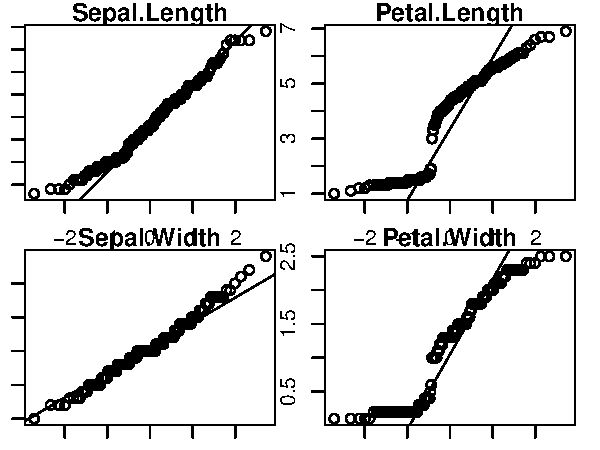
\includegraphics[width=\maxwidth]{figure/unnamed-chunk-1-1} 
\begin{kframe}\begin{verbatim}
## $Sepal.Length
## NULL
## 
## $Sepal.Width
## NULL
## 
## $Petal.Length
## NULL
## 
## $Petal.Width
## NULL
\end{verbatim}
\end{kframe}
\end{knitrout}
  \caption{1.1}
  \end{center}
  \end{figure}
  由上图可知,sepal.length与sepal.width的概率图大致均匀分布在y=x线两侧,petal.length与petal.width的图明显偏离y=x线,左边朝直线下方弯曲,右边朝直线上方弯曲,具有长尾分布的特征。
	\subsection{二维散点图}
	判定指标:通过变量间的两两散点图,如果存在不服从线性关系的两个变量,也就是散点图不成直线,则说明数据不服从多元正态分布。
	\begin{lstlisting}[language=R, caption=变量之间相关性检验,label={labelkode}]
  pairs(iris_d)  
  \end{lstlisting}
  

  \begin{figure}[H]
	\begin{center}
\begin{knitrout}
\definecolor{shadecolor}{rgb}{0.969, 0.969, 0.969}\color{fgcolor}
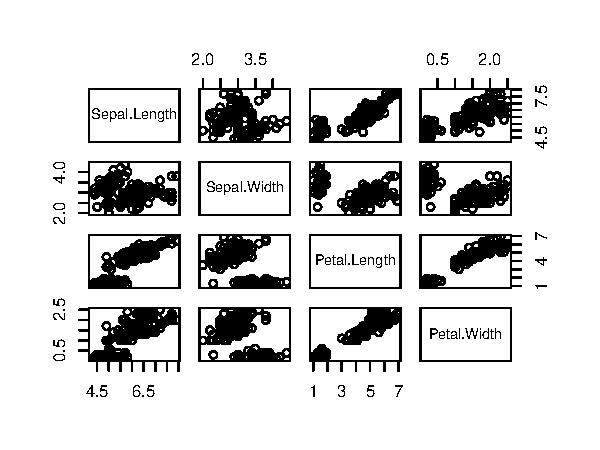
\includegraphics[width=\maxwidth]{figure/unnamed-chunk-2-1} 
\end{knitrout}
  \caption{1.2}
  \end{center}
  \end{figure}
	\subsection{马氏距离是否服从卡方分布}
		\begin{lstlisting}[language=R, caption=马氏距离卡方分布检验 ,label={labelkode}]
  y <- iris_d
cm <- colMeans(y)
S <- cov(y)
d <- apply(y, 1, function(y) t(y - cm) %*% solve(S) %*% (y - cm))
plot(qc <- qchisq((1:nrow(y) - 1/2) / nrow(y), df = 7), sd <- sort(d),
     xlab = expression(paste(chi[7]^2, " Quantile")),
     ylab = "Ordered distances", xlim = range(qc) * c(1, 1.1))
oups <- which(rank(abs(qc - sd), ties = "random") > nrow(y) - 3)
text(qc[oups], sd[oups] - 1.5, names(oups))
abline(a = 0, b = 1)
  \end{lstlisting}
		\begin{figure}[H]
\begin{center}
\begin{knitrout}
\definecolor{shadecolor}{rgb}{0.969, 0.969, 0.969}\color{fgcolor}
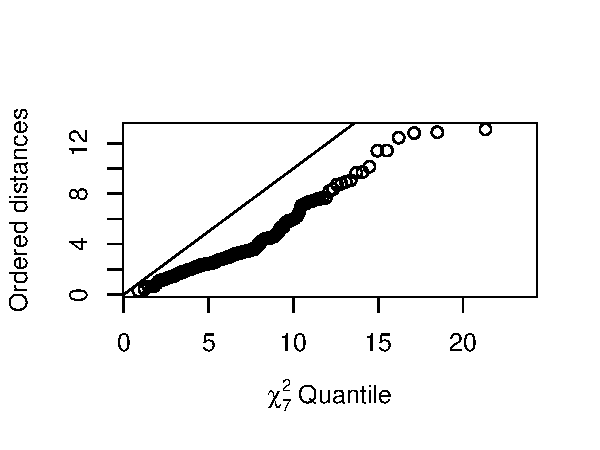
\includegraphics[width=\maxwidth]{figure/unnamed-chunk-3-1} 
\end{knitrout}
\caption{1.3}
\end{center}
\end{figure}
从qq图可以看出,点距离标准线的偏离程度较大,说明可以拒绝数据服从正态分布的假设。
  
  \subsection{夏皮罗-威尔克检验Shapiro–Wilk test}
  \begin{lstlisting}[language=R, caption=Shapiro–Wilk test,label={labelkode}]
   library(mvnormtest)
iris_d=-t(iris[,1:4])
mshapiro.test(iris_d)
  \end{lstlisting}
  		\begin{figure}[H]
      \begin{center}
\begin{knitrout}
\definecolor{shadecolor}{rgb}{0.969, 0.969, 0.969}\color{fgcolor}\begin{kframe}
\begin{verbatim}
## 
## 	Shapiro-Wilk normality test
## 
## data:  Z
## W = 0.97935, p-value = 0.02342
\end{verbatim}
\end{kframe}
\end{knitrout}
      \caption{1.4}
      \end{center}
      \end{figure}
  p-value<0.05,说明可以在0.05的水平上拒绝数据服从多元正态分布的假设。
  
	\subsection{总结}
	正态性检验在样本量不大时是有必要的,当样本量足够大时,由中心极限定理,
	不必太过纠结正态性的问题。
	\section{分类}
	使用python。
	\subsection{LDA}
	\subsubsection{降维至三维}
		\begin{lstlisting}[language=python, caption=3—dimension-LDA ,label={labelkode}]
  #导入各种程序包
import numpy as np
import pandas as pd
import seaborn as sns
import matplotlib.pyplot as plt
from sklearn.metrics import classification_report
from sklearn.discriminant_analysis import LinearDiscriminantAnalysis
clf = LinearDiscriminantAnalysis()
from sklearn.model_selection import train_test_split  
##划分训练集与测试集
from sklearn.datasets import load_iris
iris = load_iris()
X_train=iris.data
y_train=iris.target
X_train,X_test,y_train,y_test=train_test_split(X_train,y_train,
    test_size=0.4,random_state=0,stratify=y_train)
#三维(数据可视化)
def plot_LDA(converted_X,y):
    '''
    绘制经过 LDA 转换后的数据
    '''
    from mpl_toolkits.mplot3d import Axes3D
    fig=plt.figure()
    ax=Axes3D(fig)
    colors=['dodgerblue','lime','darkorange']
    target_names = iris.target_names
    markers='o*s'
 
    for target,color,marker,target_name in zip([0,1,2],colors,markers,target_names):  
        pos=(y==target).ravel() 
        X=converted_X[pos,:]
 
        ax.scatter(X[:,0], X[:,1], X[:,2],color=color,marker=marker,  
           label=target_name)
    ax.legend(loc="best")
    fig.suptitle("After LDA")
def plot_LDA1(converted_X,y):
    '''
    绘制未经 LDA 转换后的数据

    '''
    from mpl_toolkits.mplot3d import Axes3D
    fig=plt.figure()
    ax=Axes3D(fig)
    colors=['dodgerblue','lime','darkorange']
    target_names = iris.target_names
    markers='o*s'
 
    for target,color,marker,target_name in zip([0,1,2],colors,markers,target_names): 
        pos=(y==target).ravel() 
        X=converted_X[pos,:]      
 
        ax.scatter(X[:,0], X[:,1], X[:,2],color=color,marker=marker,  
           label=target_name)
    ax.legend(loc="best")
    fig.suptitle("Before LDA")
    clf.fit(X_train,y_train) 
# converted_X(150,3) 对数据降维了    权值lda.coef_(3, 4)  lda.intercept_(3,)
converted_X=np.dot(X_train,np.transpose(clf.coef_))+clf.intercept_  # X*权值+偏置b  就是输出值
plot_LDA(converted_X,y_train)
#最初未转化的三维的情况
plot_LDA1(X_train,y_train)
y_pred = clf.predict(X_test)
print(y_pred)
print(y_test)
#评估
# 分类报告:precision/recall/fi-score/均值/分类个数
from sklearn.metrics import classification_report
target_names = ['class 0', 'class 1', 'class 2']
print(classification_report(y_test, y_pred, target_names=target_names))
#准确率
from sklearn.metrics import accuracy_score
accuracy_score(y_test, y_pred)
# 混淆矩阵
from sklearn.metrics import confusion_matrix
confusion_matrix(y_test, y_pred)
  \end{lstlisting}
  运行结果:
  \begin{figure}[H]
		\centering
		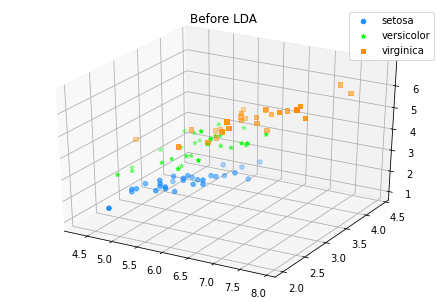
\includegraphics[width=0.8\textwidth]{Figure/LDA1.png}
		\caption{Before 3-dimension-LDA}
		\label{fig:my_label}
	\end{figure}
	\begin{figure}[H]
		\centering
		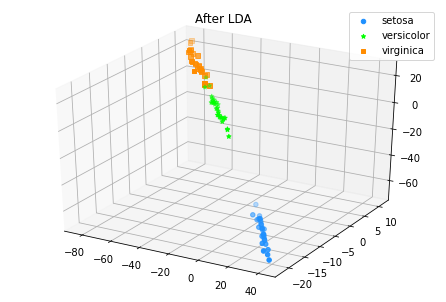
\includegraphics[width=0.8\textwidth]{Figure/LDA3.png}
		\caption{After 2-dimension-LDA}
		\label{fig:my_label}
	\end{figure}
	
	\subsubsection{降维至二维}
	大致过程与上述相同,下面只给出了关键部分的代码。
		\begin{lstlisting}[language=python, caption=2—dimension-LDA  ,label={labelkode}]
  #二维
#数据训练
lda = LinearDiscriminantAnalysis(n_components=2)
X_transform = lda.fit(X_train, y_train).transform(X_test)
y_pred = lda.predict(X_test)
#绘图
colors=['dodgerblue','lime','darkorange']
plt.figure()
target_names = iris.target_names
lw=2
for color, i, target_name in zip(colors, [0, 1, 2], target_names):
    plt.scatter(X_transform[y_pred == i, 0], X_transform[y_pred == i, 1], alpha=.8, color=color,
                label=target_name)
plt.legend(loc='best', shadow=False, scatterpoints=1)
plt.title('After 2-dimension-LDA')
plt.show()
  \end{lstlisting}
\subsubsection{运行结果}
\begin{table}[H]
		\caption{评估分类报告LDA}
		\label{tab-contoh}
		\centering
\begin{tabular}{cclll}
\textbf{} & \multicolumn{1}{l}\textbf{precision} & recall & f1-score & support \\ \cline{2-5} 
\multicolumn{1}{c|}{class 0}      & 1.00                                                           & 1.00   & 1.00     & 20      \\
\multicolumn{1}{c|}{class 1}      & 1.00                                                           & 1.00   & 1.00     & 20      \\
\multicolumn{1}{c|}{class 2}      & 1.00                                                           & 1.00   & 1.00     & 20      \\ \cline{2-5} 
\multicolumn{1}{c|}{accuracy}     & 1.00                                                           & 60     &          &         \\
\multicolumn{1}{c|}{macro avg}    & 1.00                                                           & 1.00   & 1.00     & 60      \\
\multicolumn{1}{c|}{weighted avg} & 1.00                                                           & 1.00   & 1.00     & 60     
\end{tabular}
\end{table}
\\
\begin{center}
  准确率:1.0\\
  混淆矩阵:\\

\begin{bmatrix}
	      20 & 0 & 0\\
	      0 & 20 & 0\\
	      0 & 0 & 20
	      \end{bmatrix}
\end{center}



\begin{figure}[H]
		\centering
		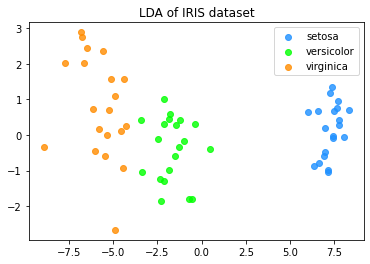
\includegraphics[width=0.8\textwidth]{Figure/LDA21.png}
		\caption{After 2-dimension-LDA}
		\label{fig:my_label}
	\end{figure}

	\subsection{SVM}
		\begin{lstlisting}[language=python, caption=SVM  ,label={labelkode}]
  #导入各种程序包
import numpy as np
import pandas as pd
import seaborn as sns
import matplotlib.pyplot as plt
from sklearn.metrics import classification_report
from sklearn.model_selection import train_test_split
from sklearn.model_selection import GridSearchCV
from sklearn.metrics import classification_report
from sklearn.svm import SVC
#网格搜索调参
tuned_parameters = [{'kernel': ['rbf'], 'gamma': [1e-3, 1e-4],
                     'C': [1, 10, 100, 1000]},
                    {'kernel': ['linear'], 'C': [1, 10, 100, 1000]}]
#评分方法定义
scores = ['precision', 'recall']
for score in scores:
    print("# Tuning hyper-parameters for %s" % score)
    print()

     # 调用 GridSearchCV,将 SVC(), tuned_parameters, cv=5, 还有 scoring 传递进去,
    clf = GridSearchCV(SVC(), tuned_parameters, cv=5, scoring='%s_macro' % score)
    # 用训练集训练这个学习器 clf
    clf.fit(X_train, y_train)

    print("Best parameters set found on development set:")
    print()

    # 再调用 clf.best_params_ 就能直接得到最好的参数搭配结果
    print(clf.best_params_)

    print()
    print("Grid scores on development set:")
    print()
    means = clf.cv_results_['mean_test_score']
    stds = clf.cv_results_['std_test_score']

    # 看一下具体的参数间不同数值的组合后得到的分数是多少
    for mean, std, params in zip(means, stds, clf.cv_results_['params']):
        print("%0.3f (+/-%0.03f) for %r"
              % (mean, std * 2, params))
    y_pred=clf.predict(X_test)
  \end{lstlisting}
\subsubsection{运行结果}
\begin{table}[H]
\caption{评估分类报告SVM}
		\label{tab-contoh}
		\centering
\begin{tabular}{cclll}
\textbf{} & \multicolumn{1}{l}\textbf{precision} & recall & f1-score & support \\ \cline{2-5} 
\multicolumn{1}{c|}{class 0}      & 1.00                                                           & 1.00   & 1.00     & 20      \\
\multicolumn{1}{c|}{class 1}      & 1.00                                                           & 0.90   & 0.95     & 20      \\
\multicolumn{1}{c|}{class 2}      & 0.91                                                           & 1.00   & 0.95     & 20      \\ \cline{2-5} 
\multicolumn{1}{c|}{accuracy}     & 0.97                                                           & 60     &          &         \\
\multicolumn{1}{c|}{macro avg}    & 0.97                                                           & 0.97   & 0.97     & 60      \\
\multicolumn{1}{c|}{weighted avg} & 0.97                                                           & 0.97   & 0.97     & 60     
\end{tabular}
\end{table}
\begin{center}
\\准确率:0.9666666666666667
\\混淆矩阵:
\\
\begin{bmatrix}
	      20 & 0 & 0\\
	      0 & 18 & 2\\
	      0 & 0 & 20
	      \end{bmatrix}
\end{center}
\subsection{总结}
从上述评估结果对比可知,LDA在iris数据集上的分类效果优于SVM的分类效果。
\end{document}


